\documentclass[a4paper, UKenglish, 11pt]{uiomaster}
\usepackage{lipsum}
\usepackage[subpreambles=true]{standalone}


\begin{document}
\chapter{Background}
Some words about what the background chapter will include.

\section{Electroencephalography}
Electroencephalography (EEG) is a non-invasively technique for studying electrical potentials in the human brain. The technique was developed almost a century ago making it among the oldest methods for examining the brain's activity. Today, EEG remains one of the most important techniques being used to study electrical activity in the brain, with important applications in both neuroscientific and clinical research (Nunez & Srinivasan 2006, Lopes da Silva 2013, Biasiucci et al. 2019, Ilmoniemi & Sarvas 2019).

EEG signal is believed to originate from large numbers of synaptic inputs to populations of geometrically aligned pyramidal neurons (Nunez & Srinivasan 2006, Pesaran et al. 2018).

Electroencephalography (EEG) is one of the most important techniques for studying cognition and disease in the brain non invasively \cite{95}. EEG is a method used to measure brain waves. In practice, this involves electrodes consisting of small metal disks connected to the surface of the scalp. The electrodes detect electrical charges that result from activity of the brain cells. In cases where certain areas of the brain come out as more active than others, it might indicate abnormalities, in which can be signs of disease. In other words, the EEG technique can be used to evaluate multiple types of brain disorders, such as lesions of the brain, Alzheimer's disease, epilepsy or brain tumors \cite{96}.

\begin{figure}[H]
    \centering
    \includegraphics[width=\linewidth]{figures/EEG_electrodes.png}
    \caption{Illustration of the EEG method \cite{97}.}
    \label{fig:EEG}
\end{figure}

An illustration of the typical EEG measurement setup is depicted in Figure \ref{fig:EEG}.

EEG signals are generated from synaptic inputs to cells in the cortex. Synaptic inputs are electrical (or chemical) signals that are being transmitted from one neuron to another, causing changes in the membrane potential of the neurons. In other words, neurons are specialized to pass signals, and synapses are the structures that make this transmission possible \cite{105}.

Imagining a small part of the cortex, all of these cells will have dendrites pointing upwards in the same direction (lets say the z-direction). Due to rotational symmetry around the z-axis, the contributions in the x- and y-direction will cancel. This is illustrated in Figure \ref{fig:EP}. What we see is that the extracellular potential is configured in all sorts of weird ways (A-C) when there is only one synaptic input, while the extracellular potential reminds more of a dipole when we have multiple synaptic inputs (D-F). We can therefore argue that the total contribution to the extracellular potential can be modelled as a dipole in the z -direction for the case where we have multiple synaptic inputs. Hence, for each dipole moment in our simulations, we pass multiple synaptic inputs, and make sure to rotate the positions of the dipoles such that it is orientated along the depth of the cortex.


\begin{figure}[H]
    \centering
    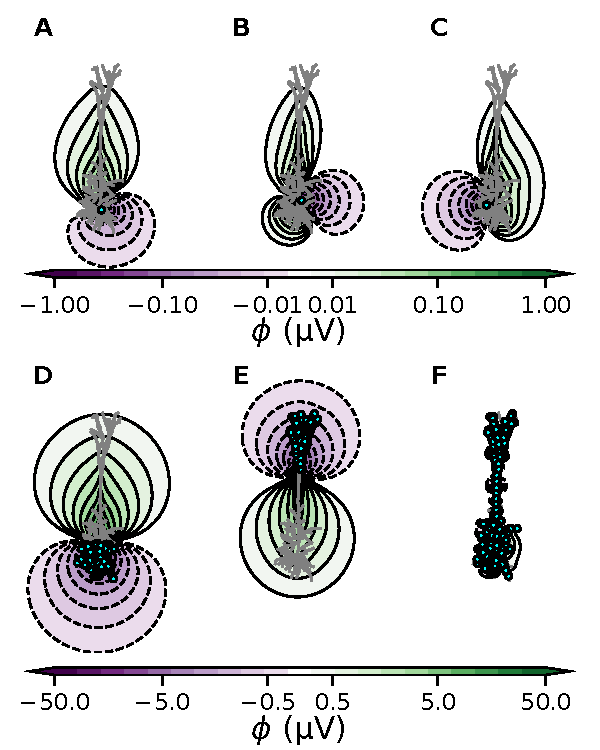
\includegraphics[width=\linewidth]{fig_chosen_dipoles.pdf}
    \caption{Extracellular potential from lonely synaptic input (A-C) and extracellular potential from multiple synaptic inputs (D-F).}
    \label{fig:EP}
\end{figure}


\section{Currend Dipoles Approximation}
EEG signals arise from cortical neural activity and are typically described in terms of current dipoles \cite{95}.

An optimal model of EEG signals would have consisted of multiple dipole moments. However, as such a model is complicated and computationally expensive, we will in this project only introduce one single dipole approximation $\textbf{p}(t)$ for each multicompartmental neuron simulation. In this context, by  multicompartmental modelling we refer to the widely used models within neuroscience, which acurately manufactures electical properties of single neurons. The sigle-dipole approximation might sound like a substantial simplification of the real biophysical properties, nevertheless it actually turns out to give a realistic modelling of EEG signals, when handling the single dipole moment, as an abnormality in the brain. We will be thinking of the abnormality as an epileptic seizures or a tumor in the brain, which among normal activity in the brain would have stuck out. The single-dipole approximation is implemented by summing up the multiple current dipole moments,
\begin{equation*}
    \textbf{p}(t) = \sum_{k=1}^M \textbf{p}_k(t) = \sum_{k=1}^M I_k^{\text{axial}}(t)\textbf{d}_k,
\end{equation*}
where $I^{\text{axial}}$ is the current flowing along the neurite with the distance vector $\textbf{d}_k$ and $M$ denotes the number of axial currents \cite{95}. The data set we will be using in this project will consist of measures of different EEG signals at a given time from 1000 patients. This means that we for each patient pick a random location (at $t=0$) for the single current dipole.

\section{The New York Head Model}
The signals received from EEG are known to originate from cortical neural activity, which are often described by using current dipoles \cite{95}. It is therefor reasonable to implement current dipoles in the brain for when generating a biophysical modeling of EEG signals. The brain model used in this thesis is called the New York Head model \cite{96}, and is based on high-resolution anatomical MRI-data from 152 adult heads. The model utilizes the software tool LFPy, which is a Python module for calculation of extracellular potentials from multicompartment neuron models \cite{100}. This model takes into account that electrical potentials are effected by the geometries and conductivities of various parts of the head \cite{95}.

The cortex matrix consists of 74382 points, which refer to the number of possible positions of the dipole moment in the cortex. When generating our data set, we will for each sample randomly pick the position of the dipole moment, such that one sample corresponds to one patient. In our head model we are considering 231 electrodes uniformly distributed across the cortex, meaning that each EEG sample will consist of this many signals for each time step. However, we are not interested in the time evolution of the signals as this does not affect nor say anything about the position of the dipole moment, and we therefor simply pick out the EEG signals for when $t$ = 0 (note that the choice of time step could have been randomly picked). Our final design matrix will then consist of 1000 rows, corresponding to each patient, and 231 columns also refereed to as features, representing the signal of each electrode. The final output we are trying to predict is then the one dimensional vector with length 1000, where each element consists of the x-, y- and z- position of the dipole moment. An example of how the input EEG signals may look like is given in appendix A, where we also have marked the dipole moment with a yellow star.

\section{The Inverse Problem and Source Localization}

% To solve the inverse EEG problem, various algorithms and methods have been developed, such as Minimum Norm Estimates (MNE), Low Resolution Electromagnetic Tomography (LORETA), and Dynamic Imaging of Coherent Sources (DICS). MACHINE LEARNIG....

% The inverse EEG problem is the problem of determining the sources of electrical activity within the brain that give rise to the measured EEG signal. The EEG signal is a recording of the electrical activity of the brain, which is measured at the surface of the scalp. However, the electrical activity that gives rise to the EEG signal is generated by a large number of sources within the brain, and it is not possible to determine the location or number of these sources just by looking at the EEG signal alone. Therefore, the inverse EEG problem is the problem of determining the sources of the EEG signal based on the measurement of the signal itself.

% To solve the inverse EEG problem, various algorithms and methods have been developed, such as Minimum Norm Estimates (MNE), Low Resolution Electromagnetic Tomography (LORETA), and Dynamic Imaging of Coherent Sources (DICS).

% However, the problem remains very challenging, as the EEG signal measured at the scalp is the result of a complex and unknown combination of sources, the brain anatomy itself and the volume conductor contribute to the complexity of the problem.

% As of now, there is not yet a definitive solution for the Inverse EEG problem and the area is still active research topic.

\end{document}